\documentclass[a4j]{jarticle}
    \usepackage[dvipdfmx]{graphicx}
    \usepackage[ top=25truemm,bottom=25truemm,left=25truemm,right=25truemm]
    {geometry}
    \usepackage{ascmac}
    \usepackage{array}
    \usepackage{here}
    \usepackage{url}
    \usepackage{listings, jlisting}
    \usepackage[subrefformat=parens]{subcaption}
    \renewcommand{\lstlistingname}{リスト}
\lstset{language=c,
  basicstyle=\ttfamily\scriptsize,
  commentstyle=\textit,
  classoffset=1,
  keywordstyle=\bfseries,
  frame=tRBl,
  framesep=5pt,
  showstringspaces=false,
  numbers=left,
  stepnumber=1,
  numberstyle=\tiny,
  tabsize=4
}

\makeatletter
\def\@thesis{プログラミング演習 レポート}
\def\id#1{\def\@id{#1}}
\def\department#1{\def\@department{#1}}

\def\@maketitle{
\begin{center}
{\huge \@thesis \par} %修士論文と記載される部分
\vspace{10mm}
{\LARGE\bf \@title \par}% 論文のタイトル部分
\vspace{10mm}
{\Large \@date\par}	% 提出年月日部分
\vspace{20mm}
{\Large \@department \par}	% 所属部分
{\Large 学籍番号 \@id \par}	% 学籍番号部分
\vspace{10mm}
{\Large 氏名 \@author}% 氏名 
\end{center}
\par\vskip 1.5em
}

\title{アナログ時計}
\date{提出期限 2020年11月24日 17:00 \\ 提出日 2020年11月24日}
\department{組番号 408}
\id{17406}
\author{金澤雄大}

    \begin{document}
    \maketitle
    \thispagestyle{empty}
    \clearpage
    \addtocounter{page}{-1}
    \section{目的}
    後期のプログラミング演習で学習した内容の理解度を確認するためにアナログ時計のアプリケーションを作成する.

    \section{実行環境}
    実行環境を\ref{env}に示す.gccとは「GNU Compiler Collection」の略称で,GNUプロジェクトが公開しているコンパイラのことである.
    makeはMakefileにプログラムのコンパイルやリンクの方法を指示することで,コンパイルを簡単に行うことができるツールのことである.
    makeを用いることは,gccコンパイル時に,長いオプションを入力しなくてよい,ファイルの更新を取得して必要なものだけをコンパイルしてくれる
    という利点がある.

    \begin{table}[H]
      \caption{実行環境}
    \label{env}
    \begin{center}
        \begin{tabular}{c|l}\hline
          CPU & Intel(R) Core(TM) i7-6500U 2.50GHz  \\ 
          メモリ & 16.0GB DDR4 \\
          OS & Microsoft Windows 10 Home \\
          gcc &  version 9.3.0 \\
          make & version 4.3 \\ \hline
        \end{tabular}
    \end{center}
    \end{table}

    \section{アプリケーションの説明}
    \label{s3}
    図\ref{clock}に示すアナログ時計のアプリケーションを作成した.
    時計の表示にはライトモードとダークモードの2種類がある.ライトモードとは白を基調とした
    画面表示のことであり,ダークモードは黒を基調とした画面表示のことである.図\ref{clock}\ref{light}はライトモードのときの時計の表示例,図\ref{clock}\ref{dark}は
    ダークモードのときの時計の表示例である.モードの切り替えは,時計アプリのウィンドウをマウスで左クリックすることで行うことができる.

        \begin{figure}[H]
          \begin{minipage}{0.5\hsize}
           \begin{center}
            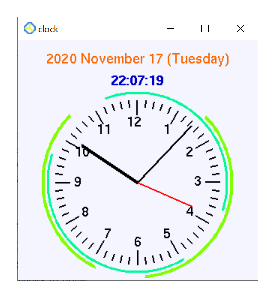
\includegraphics[scale=1.2]{light.eps}
           \end{center}
           \subcaption{ライトモードの時計}
           \label{light}
          \end{minipage}
          \begin{minipage}{0.5\hsize}
           \begin{center}
            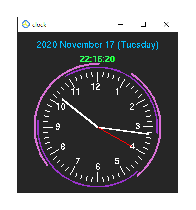
\includegraphics[scale=1.8]{dark.eps}
           \end{center}
           \subcaption{ダークモードの時計}
           \label{dark}
          \end{minipage}
          \caption{時計のアプリケーション}
          \label{clock}
         \end{figure}

          このアプリでは次に示すものを画面に描画する.アナログ時計の縁は内側と外側があり,回転している.
         回転方向は外側が時計回り,内側が反時計周りである.また,レポートでは伝わらないが,ライトモードとダークモードでは画面に描画している
         アナログ時計および文字列の色が異なる.表\ref{color}に2つのモードにおける色の設定を示す.
         \begin{itemize}
           \item アナログ時計
           \item アナログ時計の縁
           \item 年,月,日,曜日,時,分,秒の文字列 
         \end{itemize}

         \begin{table}[H]
          \caption{色の設定}
        \label{color}
        \begin{center}
            \begin{tabular}{c|c|c}\hline
              描画内容 & ライトモードでの色 & ダークモードでの色 \\ \hline
              背景色 & 白 & 黒 \\
              年 月 日(曜日) &  オレンジ & ライトブルー \\
              時:分:秒 & 青 & 緑 \\
              時計の針(分針,時針)およびインデックス & 黒 & 白 \\
              時計の針(秒針) & 赤 & 赤 \\
              時計の縁(内側) & スプリンググリーン & パープル \\
              時計の縁(外側) & ライムグリーン & ピンク \\ \hline
            \end{tabular}
        \end{center}
        \end{table}

    \section{プログラムの説明}
    \ref{s3}章で述べたアプリケーションを作成するためには次に示す機能を実装しなければならない.
    本章ではこれらを実装するプログラムの説明を行う.プログラムリスト全体については付録!を参照してほしい.
    \begin{itemize}
      \item ヘッダファイルの記述,オブジェクト形式マクロの宣言
      \item 初期化設定
      \item ウィンドウのリサイズへの対応
      \item タイマーを用いた時間の更新
      \item マウス入力の制御
      \item 画面描画の制御
      \item アナログ時計のインデックス,文字盤を表示する機能
      \item アナログ時計の針を表示する機能
      \item 年,月,日,曜日,時,分,秒の文字列を表示する機能 
    \end{itemize}

    \subsection{ヘッダファイルの記述,オブジェクト形式マクロの宣言}
    プログラムの実行に必要なヘッダファイルの記述,および必要なマクロを定義する.リスト\ref{}に
    ヘッダファイルの記述,および必要なマクロを定義したコードを示す.glut.hがc言語でOpenGLを扱う
    ためのライブラリである.また,time.hは時間の取得を行うためのライブラリである.\\
     本アプリではウィンドウサイズは320$\times$320に固定する.このため,リスト\ref{include}の8行目
    および9行目ではウィンドウのサイズを定義している.\\
     リスト\ref{include}1行目から13行目行目ではグローバル変数の定義を行っている.変数dispModeは
    ライトモード,ダークモードの管理を行うための変数である.dispModeが1のときライトモード,0のとき
    ダークモードである.変数loop1,loop2はアナログ時計の縁を回転させるための変数である.
    \begin{lstlisting}[basicstyle=\ttfamily\footnotesize, frame=single,label=include,caption=定数,変数の定義]
#include<GL/glut.h>
#include<stdio.h>
#include<time.h>
#include<math.h>
#include<string.h>

// windowのサイズを定義
#define WINDOW_W 320
#define WINDOW_H 320

int dispMode =0; // 0 : LIGHTMODE 1 : DARKMODE
double loop1=0; //use for design rotation
double loop2=0; //use for design rotation
                  \end{lstlisting}

  \subsection{初期化設定}
  メイン関数では全体の初期化および設定を行う.
  \begin{lstlisting}[basicstyle=\ttfamily\footnotesize, frame=single,label=main,caption=main関数]
int main(int argc,char **argv){
// 初期化処理
    // 引数処理
    glutInit(&argc,argv);
    // 初期Windowサイズ設定
    glutInitWindowSize(WINDOW_W,WINDOW_H);
    // 新規Window作成
    glutCreateWindow("clock");
    // 関数登録
    glutDisplayFunc(Display);
    glutReshapeFunc(Reshape);
    glutMouseFunc(Mouse);
    glutTimerFunc(500,Timer,0);
    // display初期化
    glutInitDisplayMode(GLUT_RGBA);
    if(dispMode){ // darkmodeのとき
        glClearColor(0.15,0.15,0.15,1.0);
    }else{ // lightmodeのとき
        glClearColor(0.96,0.96,1.0,1.0);
    }
    // メインループ
    glutMainLoop();
    return 0;
}
  \end{lstlisting}   

    \section{ビルド方法の説明}
    \section{実行結果とその説明}

    !付録
        \begin{thebibliography}{9}
          \bibitem{NNCT}  国立高専機構長野高専,\url{http://www.nagano-nct.ac.jp/} ,閲覧日2020年8月5日
          \end{thebibliography}
\end{document}

